\documentclass[a4paper,11pt]{report}

\usepackage{amsmath,amssymb,amsthm}
\usepackage{fullpage}
\usepackage{graphicx}

\usepackage{bussproofs}
\usepackage{mathpartir}
\usepackage{prooftrees}
\usepackage{color}
\usepackage{rotating}



\usepackage{tikz}
\usetikzlibrary{automata,positioning}
\usetikzlibrary{fit}

\newcommand*\circled[1]{\tikz[baseline=(char.base)]{
    \node[shape=circle,draw,inner sep=2pt] (char) {#1};}}

\makeatletter
\pgfmathdeclarefunction{alpha}{1}{%
  \pgfmathint@{#1}%
  \edef\pgfmathresult{\pgffor@alpha{\pgfmathresult}}%
}

\newcommand*{\until}{U}
\newcommand*{\disj}{\ ,\ }
\newcommand*{\A}{\square}  % Always
\newcommand*{\D}{\diamondsuit} % eventually

\newcommand*{\Pq}{(\top,\bot)}
\newcommand*{\pQ}{(\bot,\top)}
\newcommand*{\PQ}{(\top,\top)}
\newcommand*{\pq}{(\bot,\bot)}

\newtheorem{assumption}{Assumption}


% tikz
\usepackage{tikz}
\usetikzlibrary{snakes}



\author{Heinz Hegi, Sylvain Julmy}
\date{\today}

\setlength{\parindent}{0pt}
\setlength{\parskip}{2.5pt}

\begin{document}

\begin{center}
  \Large{
    Compiler Construction \\
    Spring 2019
  }
  
  \noindent\makebox[\linewidth]{\rule{\linewidth}{0.4pt}}
  Assignement 2 : Lexical Analysis

  \vspace*{1.4cm}

  Author : Heinz Hegi, Sylvain Julmy
  \noindent\makebox[\linewidth]{\rule{\linewidth}{0.4pt}}

  {\small
  \begin{flushright}
    Prof. Dr. O. Nierstrasz, Dr. Mohammad Ghafari \\
    Manuel Leuenberger, Rathesan Iyadurai
  \end{flushright}}

  \noindent\makebox[\linewidth]{\rule{\textwidth}{1pt}}
\end{center}

\section*{Exercise 1}

\subsection*{a)}

There exists a very simple solution but it is deterministic :

\begin{center}
  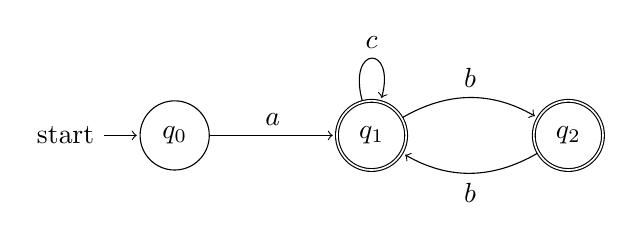
\begin{tikzpicture}[shorten >=1pt,node distance=2.5cm,on grid,auto]
    \tikzset{rounded/.style={draw,rectangle,rounded corners}}
    \node[state,initial] (q0) {$q_0$};
    \node[state,accepting] (q1) [right = of q0] {$q_1$};
    \node[state,accepting] (q2) [right = of q1] {$q_2$};
    \path[->]
    (q0)
    edge [] node [] {$a$} (q1)
    (q1)
    edge [loop above] node [] {$c$} ()
    edge [bend left] node [] {$b$} (q2)
    (q2)
    edge [bend left] node [] {$b$} (q1)
    ;
  \end{tikzpicture}
\end{center}

We also construct a NFA in order to perform the determinization algorithm :

\begin{minipage}{0.45\textwidth}
\begin{flushleft}
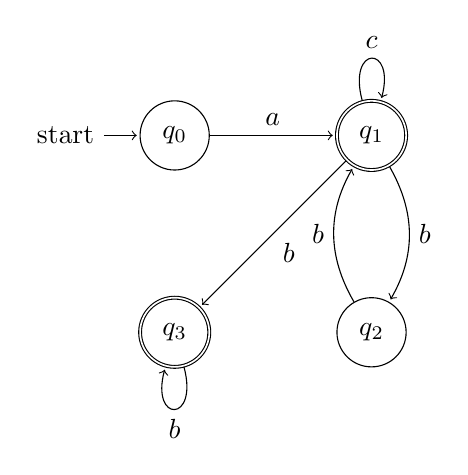
\begin{tikzpicture}[shorten >=1pt,node distance=2.5cm,on grid,auto]
  \tikzset{rounded/.style={draw,rectangle,rounded corners}}
  \node[state,initial] (q0) {$q_0$};
  \node[state,accepting] (q1) [right = of q0] {$q_1$};
  \node[state] (q2) [below = of q1] {$q_2$};
  \node[state,accepting] (q3) [below = of q0] {$q_3$};
  \path[->]
  (q0)
  edge [] node [] {$a$} (q1)
  (q1)
  edge [bend left] node [] {$b$} (q2)
  edge [] node [] {$b$} (q3)
  edge [loop above] node [] {$c$} ()
  (q2)
  edge [bend left] node [] {$b$} (q1)
  (q3)
  edge [loop below] node [] {$b$} ()
  ;
\end{tikzpicture}
\end{flushleft}
\end{minipage}
$\longmapsto$
\begin{minipage}{0.45\textwidth}
  \begin{flushright}
   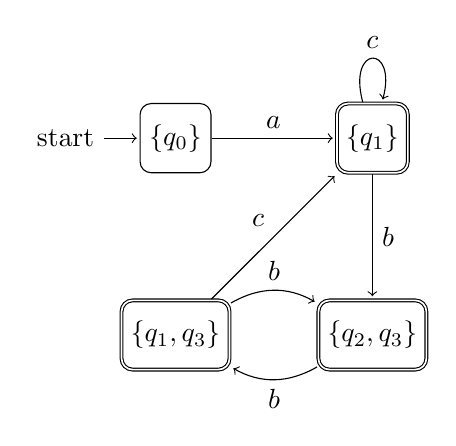
\begin{tikzpicture}[shorten >=1pt,node distance=2.5cm,on grid,auto]
    \tikzset{rounded/.style={draw,rectangle,rounded corners}}
    \node[state,rounded,initial] (q0) {$\{q_0\}$};
    \node[state,rounded,accepting] (q1) [right = of q0] {$\{q_1\}$};
    \node[state,rounded,accepting] (q2q3) [below = of q1] {$\{q_2,q_3\}$};
    \node[state,rounded,accepting] (q1q3) [left = of q2q3] {$\{q_1,q_3\}$};
    \path[->]
    (q0)
    edge [] node [] {$a$} (q1)
    (q1)
    edge [loop above] node [] {$c$} ()
    edge [] node [] {$b$} (q2q3)
    (q2q3)
    edge [bend left] node [] {$b$} (q1q3)
    (q1q3)
    edge [bend left] node [] {$b$} (q2q3)
    edge [] node [] {$c$} (q1)
    ;
  \end{tikzpicture} 
  \end{flushright}
\end{minipage}

\section*{Exercise 2}
We are going to show that the language $L = \{a^nb^n | n \geq 0\}$ over the
alphabet $\Sigma = \{a,b\}$ is not regular.

\begin{proof}
  We assume that $L$ is regular, then the Pumping Lemma for regular languages
  must hold. Let $\omega = a^nb^n$, therefore $x \in L$ and
  $|x| \leq n$. We have, by the pumping lemma, that $\exists u,v,w$ such that
  \begin{align}
    x = uvw \\
    |uv| \leq n \\
    |v| \geq 1 \\
    \forall i \geq 0 : uv^iw \in L
  \end{align}
  We show that $\forall u,v,w$, (1) to (4) don't hold. If (1) to (3) hold, then
  $x = a^nb^n = uvw$ with $|uv| \leq n$ and $|v| \geq 1$. Therefore $u=a^s$,
  $v=a^t$, $w = a^pb^n$ with $s + t \leq n$, $t \geq 1$, $p \geq 0$, $s + t + p
  = n$. But here, (4) don't hold for $i=0$ :
  $$
  uv^0w = uw = a^sa^pb^n = a^{s+p}b^n \not \in L, \text{ since $s+p \neq n$}
  $$
\end{proof}

We can also proof this less formally using the equivalence with finite
automatons. The proof is by contradiction : suppose there is a DFA $A$
(possibly converted from a NFA) with $k$ states. It implies that after $a^{k+1}$
steps, we must have visited the same state twice. Let $j$ be the number of steps
after which such a doubly visited state has been visited for the first time, and
$l$ be the number of steps to the second visit. Therefore, $A$ accepts
$a^{j+l}b^{j}$ if it accepts $a^jb^j$.

\section*{Exercise 3}

\begin{verbatim}
  b? (an)+ n? a s?
\end{verbatim}

\section*{Exercise 4}

Note that the whitespaces are just for readability. We represent the only actual
space in the regex with an underscore. The new lines and additional spaces
inside the regular expression aren't sensitive.

Solution which allows multiple spaces :

\begin{verbatim}
(([1-9][0-9]*d)                    |
 (((1[0-9])|(2[0-3])|([1-9]))h)    |
 ((([1-9])|([1-5][0-9]))(s|m))     |
 ([1-9][0-9]?[0-9]?ms)             |
 |(_))+
\end{verbatim}

Solution in which multiple spaces are not allowed :

\begin{verbatim}
(([1-9][0-9]*d)                    |
  (((1[0-9])|(2[0-3])|([1-9]))h)   |
  ([1-9][0-9]?[0-9]?ms)            |
  ((([1-9])|([1-5][0-9]))(s|m)))
(_(([1-9][0-9]*d)                  |
  (((1[0-9])|(2[0-3])|([1-9]))h)   |
  ([1-9][0-9]?[0-9]?ms)            |
  ((([1-9])|([1-5][0-9]))(s|m))))*
\end{verbatim}

\end{document}
